\documentclass[]{book}
\usepackage{lmodern}
\usepackage{amssymb,amsmath}
\usepackage{ifxetex,ifluatex}
\usepackage{fixltx2e} % provides \textsubscript
\ifnum 0\ifxetex 1\fi\ifluatex 1\fi=0 % if pdftex
  \usepackage[T1]{fontenc}
  \usepackage[utf8]{inputenc}
\else % if luatex or xelatex
  \ifxetex
    \usepackage{mathspec}
  \else
    \usepackage{fontspec}
  \fi
  \defaultfontfeatures{Ligatures=TeX,Scale=MatchLowercase}
\fi
% use upquote if available, for straight quotes in verbatim environments
\IfFileExists{upquote.sty}{\usepackage{upquote}}{}
% use microtype if available
\IfFileExists{microtype.sty}{%
\usepackage{microtype}
\UseMicrotypeSet[protrusion]{basicmath} % disable protrusion for tt fonts
}{}
\usepackage[margin=1in]{geometry}
\usepackage{hyperref}
\hypersetup{unicode=true,
            pdftitle={Quantitative Portfolio Management},
            pdfauthor={Jon Spinney},
            pdfborder={0 0 0},
            breaklinks=true}
\urlstyle{same}  % don't use monospace font for urls
\usepackage{natbib}
\bibliographystyle{apalike}
\usepackage{color}
\usepackage{fancyvrb}
\newcommand{\VerbBar}{|}
\newcommand{\VERB}{\Verb[commandchars=\\\{\}]}
\DefineVerbatimEnvironment{Highlighting}{Verbatim}{commandchars=\\\{\}}
% Add ',fontsize=\small' for more characters per line
\usepackage{framed}
\definecolor{shadecolor}{RGB}{248,248,248}
\newenvironment{Shaded}{\begin{snugshade}}{\end{snugshade}}
\newcommand{\KeywordTok}[1]{\textcolor[rgb]{0.13,0.29,0.53}{\textbf{#1}}}
\newcommand{\DataTypeTok}[1]{\textcolor[rgb]{0.13,0.29,0.53}{#1}}
\newcommand{\DecValTok}[1]{\textcolor[rgb]{0.00,0.00,0.81}{#1}}
\newcommand{\BaseNTok}[1]{\textcolor[rgb]{0.00,0.00,0.81}{#1}}
\newcommand{\FloatTok}[1]{\textcolor[rgb]{0.00,0.00,0.81}{#1}}
\newcommand{\ConstantTok}[1]{\textcolor[rgb]{0.00,0.00,0.00}{#1}}
\newcommand{\CharTok}[1]{\textcolor[rgb]{0.31,0.60,0.02}{#1}}
\newcommand{\SpecialCharTok}[1]{\textcolor[rgb]{0.00,0.00,0.00}{#1}}
\newcommand{\StringTok}[1]{\textcolor[rgb]{0.31,0.60,0.02}{#1}}
\newcommand{\VerbatimStringTok}[1]{\textcolor[rgb]{0.31,0.60,0.02}{#1}}
\newcommand{\SpecialStringTok}[1]{\textcolor[rgb]{0.31,0.60,0.02}{#1}}
\newcommand{\ImportTok}[1]{#1}
\newcommand{\CommentTok}[1]{\textcolor[rgb]{0.56,0.35,0.01}{\textit{#1}}}
\newcommand{\DocumentationTok}[1]{\textcolor[rgb]{0.56,0.35,0.01}{\textbf{\textit{#1}}}}
\newcommand{\AnnotationTok}[1]{\textcolor[rgb]{0.56,0.35,0.01}{\textbf{\textit{#1}}}}
\newcommand{\CommentVarTok}[1]{\textcolor[rgb]{0.56,0.35,0.01}{\textbf{\textit{#1}}}}
\newcommand{\OtherTok}[1]{\textcolor[rgb]{0.56,0.35,0.01}{#1}}
\newcommand{\FunctionTok}[1]{\textcolor[rgb]{0.00,0.00,0.00}{#1}}
\newcommand{\VariableTok}[1]{\textcolor[rgb]{0.00,0.00,0.00}{#1}}
\newcommand{\ControlFlowTok}[1]{\textcolor[rgb]{0.13,0.29,0.53}{\textbf{#1}}}
\newcommand{\OperatorTok}[1]{\textcolor[rgb]{0.81,0.36,0.00}{\textbf{#1}}}
\newcommand{\BuiltInTok}[1]{#1}
\newcommand{\ExtensionTok}[1]{#1}
\newcommand{\PreprocessorTok}[1]{\textcolor[rgb]{0.56,0.35,0.01}{\textit{#1}}}
\newcommand{\AttributeTok}[1]{\textcolor[rgb]{0.77,0.63,0.00}{#1}}
\newcommand{\RegionMarkerTok}[1]{#1}
\newcommand{\InformationTok}[1]{\textcolor[rgb]{0.56,0.35,0.01}{\textbf{\textit{#1}}}}
\newcommand{\WarningTok}[1]{\textcolor[rgb]{0.56,0.35,0.01}{\textbf{\textit{#1}}}}
\newcommand{\AlertTok}[1]{\textcolor[rgb]{0.94,0.16,0.16}{#1}}
\newcommand{\ErrorTok}[1]{\textcolor[rgb]{0.64,0.00,0.00}{\textbf{#1}}}
\newcommand{\NormalTok}[1]{#1}
\usepackage{longtable,booktabs}
\usepackage{graphicx,grffile}
\makeatletter
\def\maxwidth{\ifdim\Gin@nat@width>\linewidth\linewidth\else\Gin@nat@width\fi}
\def\maxheight{\ifdim\Gin@nat@height>\textheight\textheight\else\Gin@nat@height\fi}
\makeatother
% Scale images if necessary, so that they will not overflow the page
% margins by default, and it is still possible to overwrite the defaults
% using explicit options in \includegraphics[width, height, ...]{}
\setkeys{Gin}{width=\maxwidth,height=\maxheight,keepaspectratio}
\IfFileExists{parskip.sty}{%
\usepackage{parskip}
}{% else
\setlength{\parindent}{0pt}
\setlength{\parskip}{6pt plus 2pt minus 1pt}
}
\setlength{\emergencystretch}{3em}  % prevent overfull lines
\providecommand{\tightlist}{%
  \setlength{\itemsep}{0pt}\setlength{\parskip}{0pt}}
\setcounter{secnumdepth}{5}
% Redefines (sub)paragraphs to behave more like sections
\ifx\paragraph\undefined\else
\let\oldparagraph\paragraph
\renewcommand{\paragraph}[1]{\oldparagraph{#1}\mbox{}}
\fi
\ifx\subparagraph\undefined\else
\let\oldsubparagraph\subparagraph
\renewcommand{\subparagraph}[1]{\oldsubparagraph{#1}\mbox{}}
\fi

%%% Use protect on footnotes to avoid problems with footnotes in titles
\let\rmarkdownfootnote\footnote%
\def\footnote{\protect\rmarkdownfootnote}

%%% Change title format to be more compact
\usepackage{titling}

% Create subtitle command for use in maketitle
\newcommand{\subtitle}[1]{
  \posttitle{
    \begin{center}\large#1\end{center}
    }
}

\setlength{\droptitle}{-2em}
  \title{Quantitative Portfolio Management}
  \pretitle{\vspace{\droptitle}\centering\huge}
  \posttitle{\par}
  \author{Jon Spinney}
  \preauthor{\centering\large\emph}
  \postauthor{\par}
  \predate{\centering\large\emph}
  \postdate{\par}
  \date{2018-03-10}

\usepackage{booktabs}
\usepackage{amsthm}
\makeatletter
\def\thm@space@setup{%
  \thm@preskip=8pt plus 2pt minus 4pt
  \thm@postskip=\thm@preskip
}
\makeatother

\usepackage{amsthm}
\newtheorem{theorem}{Theorem}[chapter]
\newtheorem{lemma}{Lemma}[chapter]
\theoremstyle{definition}
\newtheorem{definition}{Definition}[chapter]
\newtheorem{corollary}{Corollary}[chapter]
\newtheorem{proposition}{Proposition}[chapter]
\theoremstyle{definition}
\newtheorem{example}{Example}[chapter]
\theoremstyle{definition}
\newtheorem{exercise}{Exercise}[chapter]
\theoremstyle{remark}
\newtheorem*{remark}{Remark}
\newtheorem*{solution}{Solution}
\begin{document}
\maketitle

{
\setcounter{tocdepth}{1}
\tableofcontents
}
\chapter{Preliminary Material}\label{preliminary-material}

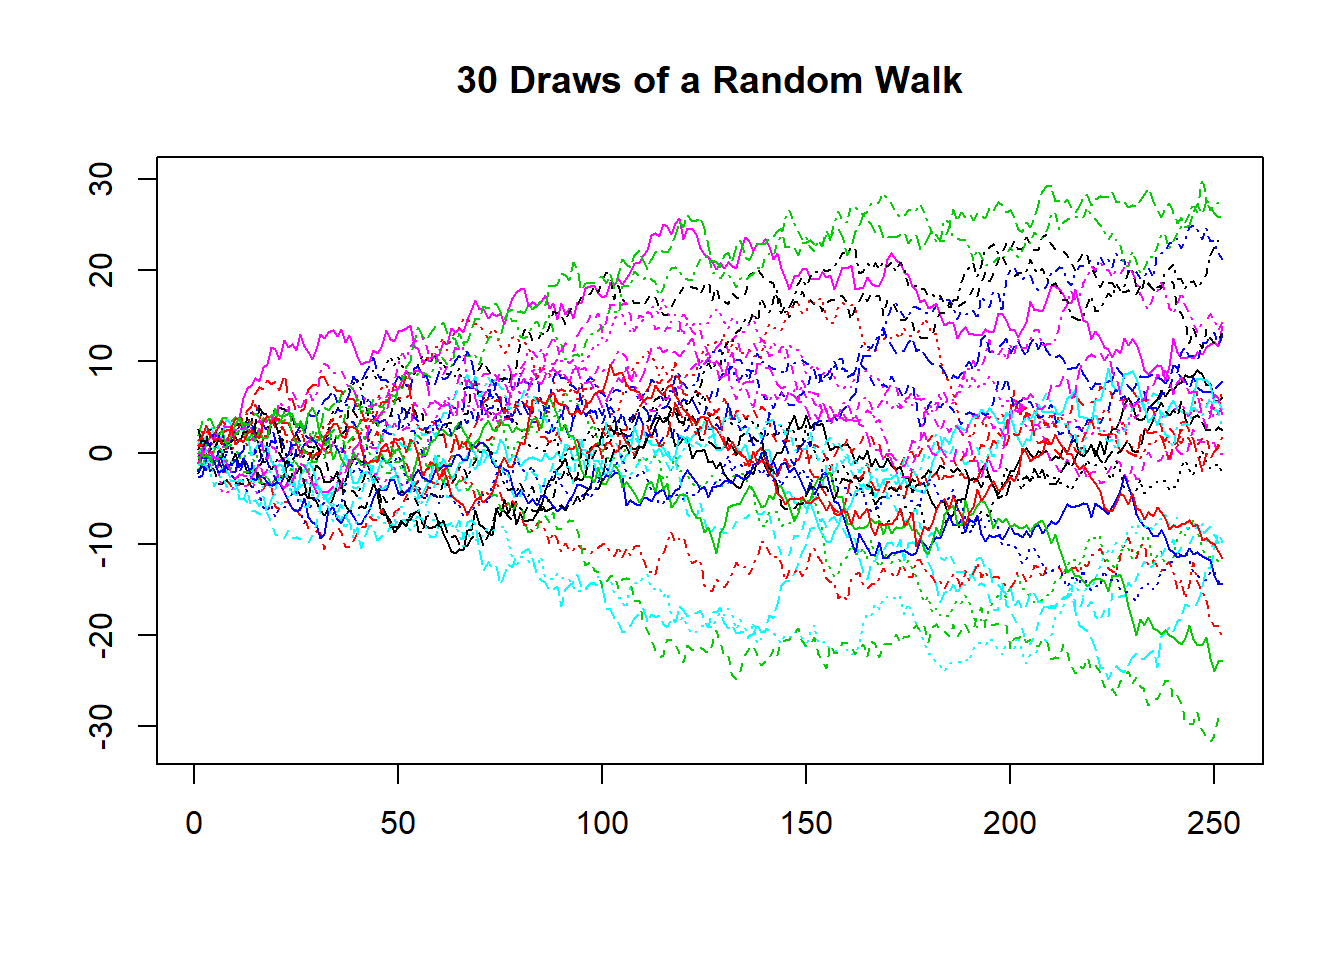
\includegraphics{mqim_book_files/figure-latex/unnamed-chunk-1-1.pdf}

This book contains the course notes for the class \textbf{MQIM 6604 -
Quantitative Portfolio Management} for the Master in Quantitative
Investment Management (MQIM) at the University of New Brunswick. All
required reading material for the course is contained in this book
(there is no other required textbook).

\chapter{Introduction}\label{intro}

This book contains course notes supporting the class MQIM 6604 -
Quantitative Portfolio Management in the Master in Quantitative
Investment Management (MQIM) at the University of New Brunswick in
Fredericton. This book, in addition to the slides and supplementary
reading assigned in lectures, are the only material required for the
class.

While there are a plethora of commercially available books related to
the field of quantitative equity portfolio management, this book
contains a few primary advantages for MQIM students. Namely:

\begin{itemize}
\tightlist
\item
  The book is new, and constantly evolving, allowing it to continually
  reflect the current practice of quantitative investment management in
  the field today. While \citep{grinold2000} may be considered the
  longstanding ``bible'' of active quantitative equity portfolio
  management and would be an excellent addition to the bookshelf of any
  practicing quant, it was last updated nearly 20 years ago.
\item
  The book is targeted to be at exactly the correct level for students
  in the MQIM program, immediately working with appropriate levels of
  mathematical sophistication for the technically minded students in the
  program. Conversely, commercially available texts may be at a level
  that is too low or two high for the MQIM program.
\item
  The R language (which is the primary language of instruction in the
  UNB MQIM program) is embedded throughout the book, and indeed the book
  is written in R using markdown and the Bookdown package
  \citep{xie2015}, making this the only book on quantitative equity
  portfolio management to make such extensive use of R.
\end{itemize}

\section{Commercially Available Textbooks Related to Quantitative Equity
Portfolio
Management}\label{commercially-available-textbooks-related-to-quantitative-equity-portfolio-management}

Students that are particularly interested in the field (or are looking
for additional companion material to help with 6604) could look at any
of the following books:

\textbf{Active Portfolio Management: A Quantitative Approach for
Producing Superior Returns and Controlling Risk} \citep{grinold2000}

\begin{itemize}
\tightlist
\item
  \url{https://www.amazon.ca/Active-Portfolio-Management-Quantitative-Controlling/dp/0070248826}
\item
  Generally considered to be the ``bible'' of quantitative equity
  portfolio management - contains early references to the authors' work
  on the Fundamental Law of Active Management. Essential reading for
  practicing quants.
\end{itemize}

\textbf{Risk and Asset Allocation} \citep{meucci2005}

\begin{itemize}
\tightlist
\item
  \url{https://www.amazon.ca/Risk-Asset-Allocation-Attilio-Meucci/dp/3642009646/}
\item
  Quite technical and idiosyncratic in its approach. The author provides
  a significant amount of Matlab code related to book examples
  (partially ported to R in the \textbf{meucci} packge) and runs an
  annual 1-week \textbf{Advanced Risk and Portfolio Management
  (``ARPM'')} bootcamp in New York every summer
  \url{https://www.arpm.co/bootcamp/}
\end{itemize}

\textbf{Quantitative Equity Portfolio Management: An Active Approach to
Portfolio Construction and Management} \citep{chincarini2006}

\begin{itemize}
\tightlist
\item
  \url{https://www.amazon.ca/Quantitative-Equity-Portfolio-Management-Construction/dp/0071459391/}
\item
  Targeted at MBA students.
\end{itemize}

\textbf{Quantitative Equity Portfolio Management: Modern Techniques and
Applications} \citep{qian2007}

\begin{itemize}
\tightlist
\item
  \url{https://www.amazon.ca/Quantitative-Equity-Portfolio-Management-Applications/dp/1584885580/}
\item
  More advanced and more modern than \citep{grinold2000}, a good read
  for practicing quants.
\end{itemize}

\textbf{Quantitative Equity Investing: Techniques and Strategies}
\citep{fabozzi2010}

\begin{itemize}
\tightlist
\item
  \url{https://www.amazon.ca/Quantitative-Equity-Investing-Techniques-Strategies/dp/0470262478/}
\end{itemize}

\textbf{Modern Investment Management: An Equilibrium Approach}
\citep{litterman2003}

\begin{itemize}
\tightlist
\item
  \url{https://www.amazon.ca/Modern-Investment-Management-Equilibrium-Approach/dp/0471124109/}
\item
  Written/edited by Robert Litterman and the (at that time) Quantitative
  Strategies Group of Goldman Sachs Asset Management.
\end{itemize}

\textbf{Asset Management: A Systematic Approach to Factor Investing}
\citep{ang2014}

\begin{itemize}
\tightlist
\item
  \url{https://www.amazon.ca/Asset-Management-Systematic-Approach-Investing/dp/0199959323/}
\item
  The most recent of all the commercially available books on this list,
  this book is non-technical (appropriate for MBA \& business school
  Undergraduate students) but makes an excellent companion book forMQIM
  6604 student for extra explanatory material and practical real-world
  examples of many applications of factor investing and quantitative
  approaches to portfolio management in general.
\end{itemize}

\section{Course Description and Background
Information}\label{course-description-and-background-information}

TBC

test table using kable:

\begin{Shaded}
\begin{Highlighting}[]
\NormalTok{knitr}\OperatorTok{::}\KeywordTok{kable}\NormalTok{(}
  \KeywordTok{head}\NormalTok{(mtcars[, }\DecValTok{1}\OperatorTok{:}\DecValTok{8}\NormalTok{], }\DecValTok{10}\NormalTok{), }\DataTypeTok{booktabs =} \OtherTok{TRUE}\NormalTok{,}
  \DataTypeTok{caption =} \StringTok{'A table of the first 10 rows of the mtcars data.'}
\NormalTok{)}
\end{Highlighting}
\end{Shaded}

\begin{table}

\caption{\label{tab:unnamed-chunk-3}A table of the first 10 rows of the mtcars data.}
\centering
\begin{tabular}[t]{lrrrrrrrr}
\toprule
  & mpg & cyl & disp & hp & drat & wt & qsec & vs\\
\midrule
Mazda RX4 & 21.0 & 6 & 160.0 & 110 & 3.90 & 2.620 & 16.46 & 0\\
Mazda RX4 Wag & 21.0 & 6 & 160.0 & 110 & 3.90 & 2.875 & 17.02 & 0\\
Datsun 710 & 22.8 & 4 & 108.0 & 93 & 3.85 & 2.320 & 18.61 & 1\\
Hornet 4 Drive & 21.4 & 6 & 258.0 & 110 & 3.08 & 3.215 & 19.44 & 1\\
Hornet Sportabout & 18.7 & 8 & 360.0 & 175 & 3.15 & 3.440 & 17.02 & 0\\
\addlinespace
Valiant & 18.1 & 6 & 225.0 & 105 & 2.76 & 3.460 & 20.22 & 1\\
Duster 360 & 14.3 & 8 & 360.0 & 245 & 3.21 & 3.570 & 15.84 & 0\\
Merc 240D & 24.4 & 4 & 146.7 & 62 & 3.69 & 3.190 & 20.00 & 1\\
Merc 230 & 22.8 & 4 & 140.8 & 95 & 3.92 & 3.150 & 22.90 & 1\\
Merc 280 & 19.2 & 6 & 167.6 & 123 & 3.92 & 3.440 & 18.30 & 1\\
\bottomrule
\end{tabular}
\end{table}

\section{Introduction to R \& Exploratory Data
Analysis}\label{introduction-to-r-exploratory-data-analysis}

TBC

\chapter{Modern Portfolio Theory}\label{mpt}

Notes:

\begin{itemize}
\tightlist
\item
  Derive eff front \& cal
\item
  equilibrium expected returns
\end{itemize}

\section{Markowitz}\label{markowitz}

TBC

\section{CAPM}\label{capm}

Notes:

\begin{itemize}
\tightlist
\item
  TBC
\end{itemize}

\section{APT \& Multifactor Models}\label{apt-multifactor-models}

TBC

\section{Modern Approaches}\label{modern-approaches}

TBC

\chapter{Anomalies \& Alpha Strategies}\label{anomalies}

TBC

\section{Early Anomalies Literature}\label{early-anomalies-literature}

TBC

\section{Fama French (1990s)}\label{fama-french-1990s}

TBC

\section{Carhart}\label{carhart}

TBC

\section{Other Factors}\label{other-factors}

BAB, QMJ, Fama French 2000s

\chapter{Forecasting}\label{forecasting}

TBC

\section{Fractile Zero-Investment
Portfolios}\label{fractile-zero-investment-portfolios}

TBC

\section{Factor Mimicking Portfolios}\label{factor-mimicking-portfolios}

TBC

\section{Fama-Macbeth Regressions}\label{fama-macbeth-regressions}

TBC

\section{Optimal Predictors}\label{optimal-predictors}

TBC

\chapter{Portfolio Optimization}\label{portopt}

TBC

\section{Minimum Variance Portfolios}\label{minimum-variance-portfolios}

TBC

\subsection{Case Study: Minimum Variance
Portfolios}\label{case-study-minimum-variance-portfolios}

TBC

\section{Constrained Optimization}\label{constrained-optimization}

TBC

\section{Active Portfolio
Optimization}\label{active-portfolio-optimization}

TBC

\section{Modern Optimization}\label{modern-optimization}

TBC

\chapter{Risk Models}\label{risk}

TBC

\section{Risk Measures}\label{risk-measures}

\begin{itemize}
\tightlist
\item
  Variance \& Volatility
\item
  Semi-deviation
\item
  VaR
\item
  CVaR
\end{itemize}

\section{Covariance Matrices and Bayesian Shrinkage
Models}\label{covariance-matrices-and-bayesian-shrinkage-models}

TBC

\section{Principal Components
Analysis}\label{principal-components-analysis}

TBC

\section{Fundamental Factor Models}\label{fundamental-factor-models}

TBC

\begin{itemize}
\tightlist
\item
  Ex 1: Single Index Model
\item
  Ex 2: Industry MOdel
\item
  Ex 3: Barra Style Model
\end{itemize}

\chapter{Post-Modern Portfolio Theory}\label{pmpt}

The original Markowitz spproach to portfolio construction, which we
implemented via the Quadratic Utility approach of:

\[
max_\omega \quad \omega' \mu - 2^{-1}\lambda^{-1} \omega' \Sigma \omega \quad \text{s.t.} \ \omega' \mathbf{1} = 1
\]

is typically referred to as \textbf{Modern Portfolio Theory (``MPT'')}.
MPT requires the estimation of asset means and co-variances, and trades
off return vs.~risk in an optimization framework. While the approach is
intuitive in its approach, practitioners have found numerous challenges
in the implementation of the MPT framework, including:

\begin{itemize}
\tightlist
\item
  unintuitive holdings,
\item
  highly concentrated portfolios, and
\item
  excess turnover.
\end{itemize}

Each of these issues leads to a common phenomenon of MTP optimal
portfolios producing inferior results out of sample relative to more
naive approaches. A significant contributor to the challenge of
implementing MPT approaches is the combination of the extreme
sensitivity of the MPT approach to errors in the mean vector, combined
with the real-world challenge of estimating such a noisy parameter. This
extreme sensitivity arises as a result of the \emph{full investment
constraint} in the optimization process. These challenges have resulted
in numerous adaptations of the MPT approach in practice, including:

\begin{itemize}
\tightlist
\item
  Risk Parity Investing,
\item
  Diversification/Concentration Management, and
\item
  Alternative Risk Definitions (e.g.~Mean-CVaR) that focus on downside
  risk as opposed to the symmatric nature of variance/volatility.
\end{itemize}

Collectively, these and other more recent approaches to portfolio
construction can be referred to as \textbf{Post-Modern Portfolio Theory
(``PMPT'')}.

\section{Risk Parity}\label{risk-parity}

Risk parity terminology and meaning often depends on the user, but for
the purposes of this book, we define two classes of risk parity
approaches to investing - \textbf{inverse volatility (``IV'')}, which is
sometimes also referred to as \emph{naive risk parity}, and
\textbf{equal risk contribution (``ERC'')}. IV as a weighting scheme
that weights securities or asset classes proportional to the inverse of
their volatility, whereas ERC is a more complicated approach to
portfolio construction that results each security's contribution to
total portfolio risk being equal. IV strategies therefore consider only
the volatilities of the assets in the universe, while ERC strategies
consider also the covariance structure between all the assets in the
portfolio.

As a visualization, consider a standard 60-40 portfolio of stocks and
bonds. Using recent data, the volatility of the equity portion was about
10\%, while the volatility of the bond portfolio was closer to 3.5\% -
the portfolio itself had to total combined volatility of about 6\% (the
correlation between bonds and stocks during this period was 0). How much
of the portfolio total volatility could be attributed to the two
components?

\begin{longtable}[]{@{}lccc@{}}
\toprule
Asset Class & Weight (\%) & Volatility (\%) & \% Contrib. to Port
Risk\tabularnewline
\midrule
\endhead
Equities & 60\% & 10.2\% & 99.4\%\tabularnewline
Bonds & 40\% & 3.5\% & 0.6\%\tabularnewline
Total Portfolio & 100\% & 6.3\% & 100\%\tabularnewline
\bottomrule
\end{longtable}

Consider instead if we had used a portfolio approach that sought to
equalize the \textbf{\% Contrib. to Port Risk} at 50\% for each asset
class:

\begin{longtable}[]{@{}lccc@{}}
\toprule
Asset Class & Weight (\%) & Volatility (\%) & \% Contrib. to Port
Risk\tabularnewline
\midrule
\endhead
Equities & 25.5\% & 10.2\% & 50\%\tabularnewline
Bonds & 74.5\% & 3.5\% & 50\%\tabularnewline
Total Portfolio & 100\% & 3.7\% & 100\%\tabularnewline
\bottomrule
\end{longtable}

The \textbf{Equal Risk Contribution} portfolio has just 25\% of its
assets in the higher risk equity portfolio and 75\% of its assets in the
relatively lower volatility bond portfolio. The portfolio, with a total
risk of 3.7\%, derives 50\% of its volatility from bonds and 50\% from
equities.

There are two main quantitative approaches to risk parity - naive risk
parity that ignores correlations and weights stocks proportionally to
the inverse of their volatility forecasts and equal risk contribution
portfolios that take into account the full covariance structure of the
market in setting the \% Contrib. to Port Risk to be equal for all
assets.

\subsection{Inverse Volatility Weighting (Naive Risk
Parity)}\label{inverse-volatility-weighting-naive-risk-parity}

For IV, we first estimate the volatility of the assets in the universe
and then assign weights to each asset in the resulting portfolio such
that:

\[
\omega_i = \frac{\sigma^{-1}_i}{\sum_{i=1}^k \sigma^{-1}_i}
\]

In the IV portfolio construction process, assets with lower volatilities
are assigned higher weights, and assets with higher volatilities are
assigned lower weights.

\begin{Shaded}
\begin{Highlighting}[]
\KeywordTok{library}\NormalTok{(quantmod)}
\NormalTok{tickers <-}\StringTok{ }\KeywordTok{c}\NormalTok{(}\StringTok{"F"}\NormalTok{,}\StringTok{"MMM"}\NormalTok{,}\StringTok{"MSFT"}\NormalTok{)}
\KeywordTok{getSymbols}\NormalTok{(tickers)}
\end{Highlighting}
\end{Shaded}

\begin{verbatim}
## [1] "F"    "MMM"  "MSFT"
\end{verbatim}

\begin{Shaded}
\begin{Highlighting}[]
\NormalTok{dat <-}\StringTok{ }\KeywordTok{merge.xts}\NormalTok{(F}\OperatorTok{$}\NormalTok{F.Adjusted, MMM}\OperatorTok{$}\NormalTok{MMM.Adjusted, MSFT}\OperatorTok{$}\NormalTok{MSFT.Adjusted)}
\NormalTok{ret <-}\StringTok{ }\NormalTok{(}\KeywordTok{exp}\NormalTok{(}\KeywordTok{diff}\NormalTok{(}\KeywordTok{log}\NormalTok{(dat)))}\OperatorTok{-}\DecValTok{1}\NormalTok{)[}\OperatorTok{-}\DecValTok{1}\NormalTok{,]}
\NormalTok{vols <-}\StringTok{ }\KeywordTok{apply}\NormalTok{(ret,}\DecValTok{2}\NormalTok{,sd)}
\NormalTok{wgts_rp <-}\StringTok{ }\NormalTok{(}\DecValTok{1}\OperatorTok{/}\NormalTok{vols)}\OperatorTok{/}\KeywordTok{sum}\NormalTok{(}\DecValTok{1}\OperatorTok{/}\NormalTok{vols)}
\KeywordTok{names}\NormalTok{(wgts_rp) <-}\StringTok{ }\NormalTok{tickers}
\KeywordTok{barplot}\NormalTok{(wgts_rp,}
        \DataTypeTok{main=}\StringTok{"Weights of Naive Risk Parity Portfolio for F, MMM and MSFT"}\NormalTok{,}
        \DataTypeTok{xlab=}\StringTok{"Stock"}\NormalTok{,}
        \DataTypeTok{ylab=}\StringTok{"Weight in Portfolio"}\NormalTok{)}
\end{Highlighting}
\end{Shaded}

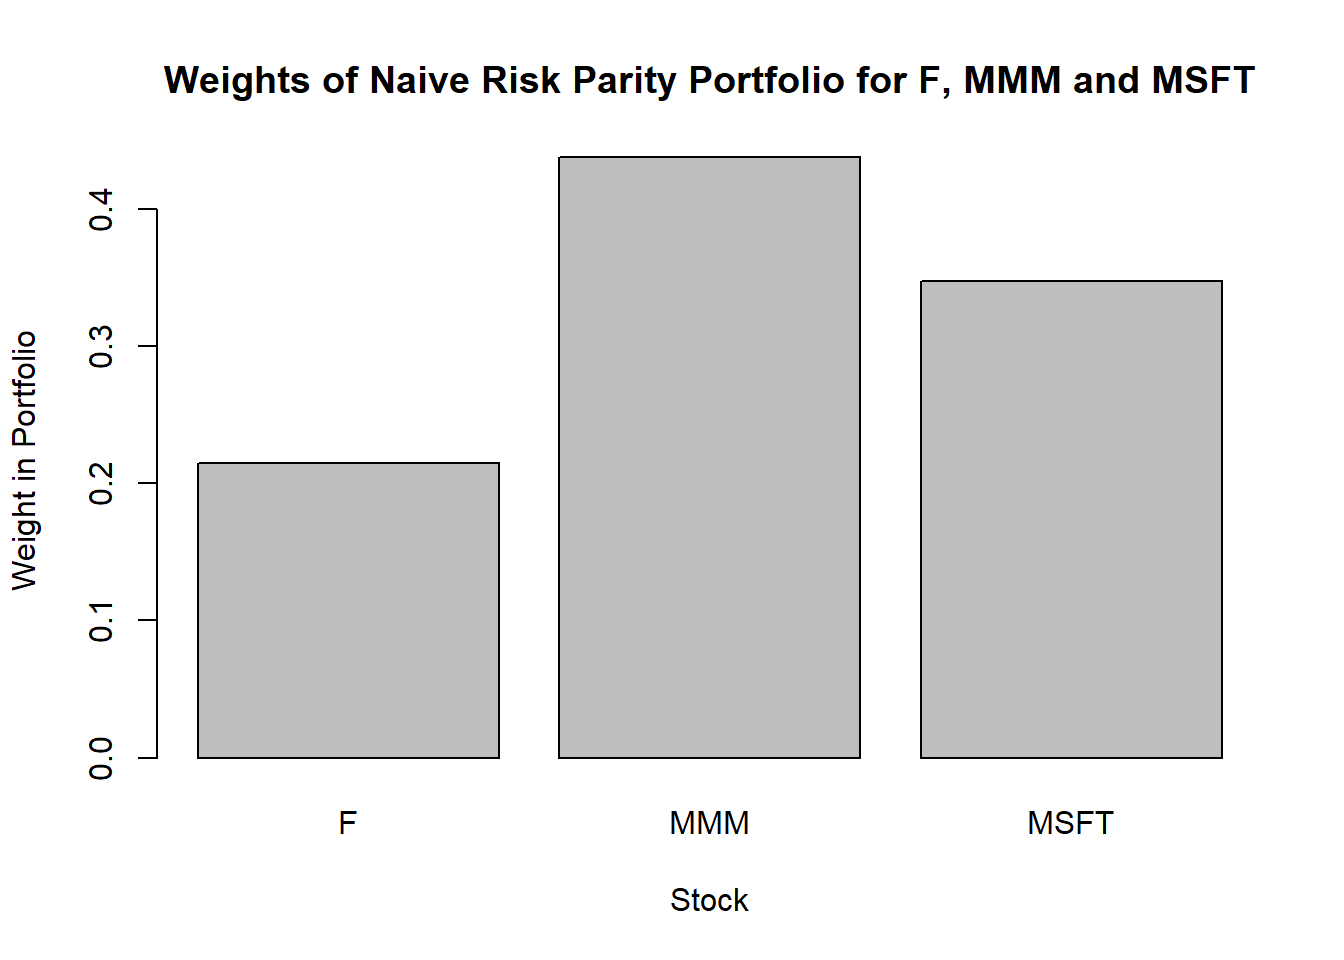
\includegraphics{mqim_book_files/figure-latex/unnamed-chunk-4-1.pdf}

\subsection{Equal Risk Contributions}\label{equal-risk-contributions}

A more complicated approach to risk parity is the one that chooses asset
weights such that the contribution of each asset to the total
portfolio's risk is equal. Like IV approaches, ERC applies relatively
higher weights to lower risk assets and vice versa, but unlike IV
approaches, the ERC methodology considers the full covariance structure
of the market, not just the asset variances.

The ERC approac of \citep{maillard2010} requires a solution to the
following:

\[
TRC_i = TRC_j \quad \forall_{i,j}
\]

Where

\[
TRC_i = \omega_i \frac{\partial \sigma_p}{\partial \omega_i}
\]

This ERC problem can be solved via a newton approach (Algorithm 1 in
\citep{chaves2012}). The R function \textbf{SolveRiskParity()} computes
ERC portfolio weights for a given covariance matrix (function code not
shown).

\begin{Shaded}
\begin{Highlighting}[]
\KeywordTok{library}\NormalTok{(tseries)}
\KeywordTok{library}\NormalTok{(quantmod)}
\NormalTok{tickers <-}\StringTok{ }\KeywordTok{c}\NormalTok{(}\StringTok{"F"}\NormalTok{,}\StringTok{"MMM"}\NormalTok{,}\StringTok{"MSFT"}\NormalTok{)}
\KeywordTok{getSymbols}\NormalTok{(tickers)}
\end{Highlighting}
\end{Shaded}

\begin{verbatim}
## [1] "F"    "MMM"  "MSFT"
\end{verbatim}

\begin{Shaded}
\begin{Highlighting}[]
\NormalTok{dat <-}\StringTok{ }\KeywordTok{merge.xts}\NormalTok{(F}\OperatorTok{$}\NormalTok{F.Adjusted, MMM}\OperatorTok{$}\NormalTok{MMM.Adjusted, MSFT}\OperatorTok{$}\NormalTok{MSFT.Adjusted)}
\NormalTok{ret <-}\StringTok{ }\NormalTok{(}\KeywordTok{exp}\NormalTok{(}\KeywordTok{diff}\NormalTok{(}\KeywordTok{log}\NormalTok{(dat)))}\OperatorTok{-}\DecValTok{1}\NormalTok{)[}\OperatorTok{-}\DecValTok{1}\NormalTok{,]}
\NormalTok{sigma <-}\StringTok{ }\KeywordTok{cov}\NormalTok{(ret)}
\NormalTok{erc_soln <-}\StringTok{ }\KeywordTok{SolveRiskParity}\NormalTok{(sigma)}
\NormalTok{wgts <-}\StringTok{ }\NormalTok{erc_soln}\OperatorTok{$}\NormalTok{port_wgt[,}\DecValTok{1}\NormalTok{]}
\KeywordTok{names}\NormalTok{(wgts) <-}\StringTok{ }\NormalTok{tickers}
\KeywordTok{barplot}\NormalTok{(wgts,}
        \DataTypeTok{main=}\StringTok{"Weights of ERC Portfolio for F, MMM and MSFT"}\NormalTok{,}
        \DataTypeTok{xlab=}\StringTok{"Stock"}\NormalTok{,}
        \DataTypeTok{ylab=}\StringTok{"Weight in Portfolio"}\NormalTok{)}
\end{Highlighting}
\end{Shaded}

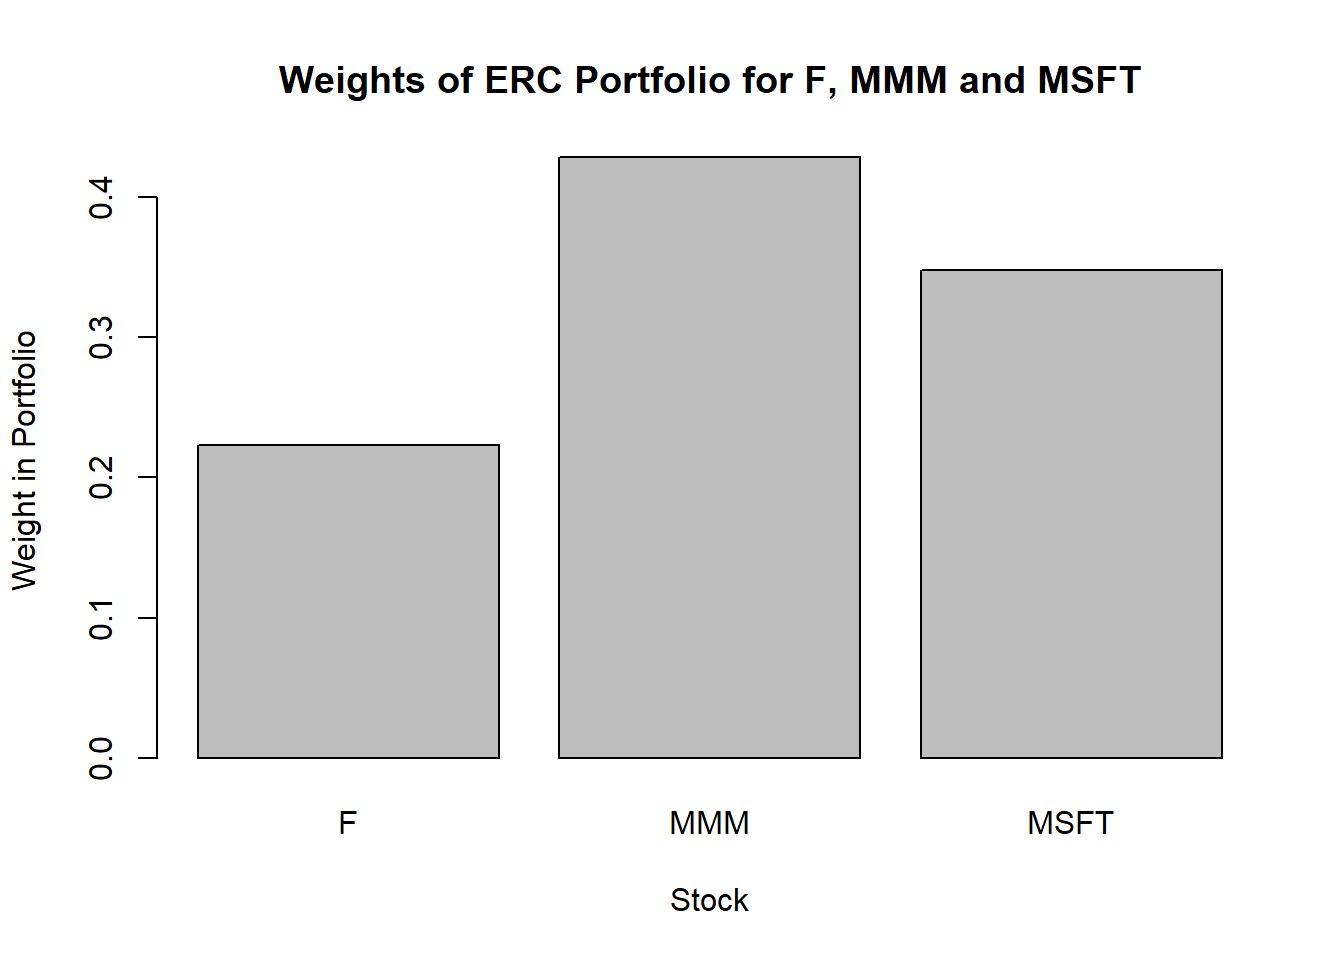
\includegraphics{mqim_book_files/figure-latex/unnamed-chunk-6-1.pdf}

We can confirm that the risk contribution is equal for each asset by
verifying that
\(\omega_i \times \frac{\partial \sigma_p}{\partial \omega_i} = \omega_j \times \frac{\partial \sigma_p}{\partial \omega_j} \quad \forall \ i, j\):

\begin{Shaded}
\begin{Highlighting}[]
\NormalTok{contribs <-}\StringTok{ }\NormalTok{erc_soln}\OperatorTok{$}\NormalTok{pctr[,}\DecValTok{1}\NormalTok{]}
\KeywordTok{names}\NormalTok{(contribs) <-}\StringTok{ }\NormalTok{tickers}
\KeywordTok{barplot}\NormalTok{(contribs,}
        \DataTypeTok{main=}\StringTok{"Pct. Contrib to Port. Risk of ERC Portfolio for F, MMM and MSFT"}\NormalTok{,}
        \DataTypeTok{xlab=}\StringTok{"Stock"}\NormalTok{,}
        \DataTypeTok{ylab=}\StringTok{"PCTR"}\NormalTok{)}
\end{Highlighting}
\end{Shaded}

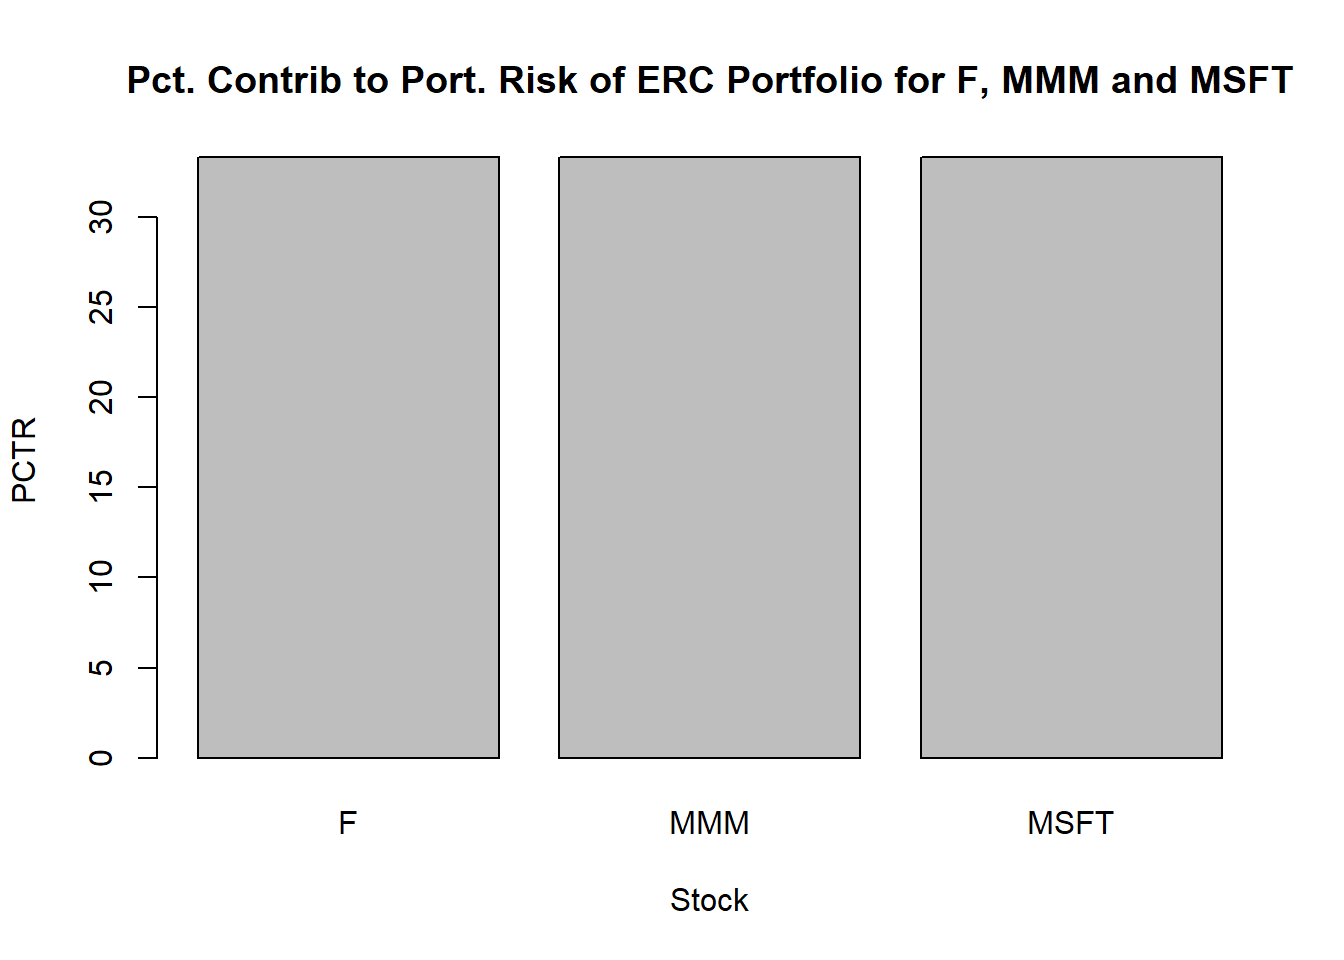
\includegraphics{mqim_book_files/figure-latex/unnamed-chunk-7-1.pdf}

In general, ERC portfolios have reduced risk relative to a market
capitalization weighted or equally weighted benchmark due to the
relative overweighting of assets with lower volatility and relative
underweighting of assets with relatively higher volatility - there is on
average a negative relationship between an asset's volatility and its
weight in the ERC portfolio:

\begin{Shaded}
\begin{Highlighting}[]
\KeywordTok{library}\NormalTok{(calibrate)}
\NormalTok{vols <-}\StringTok{ }\KeywordTok{apply}\NormalTok{(ret,}\DecValTok{2}\NormalTok{,sd)}\OperatorTok{*}\KeywordTok{sqrt}\NormalTok{(}\DecValTok{252}\NormalTok{)}
\KeywordTok{plot}\NormalTok{(vols,wgts,}
     \DataTypeTok{main=}\StringTok{"Stock Volatility vs. Weight in ERC Portfolio"}\NormalTok{,}
     \DataTypeTok{xlab=}\StringTok{"Volatility"}\NormalTok{,}
     \DataTypeTok{ylab=}\StringTok{"Weight in Portfolio"}\NormalTok{,}
     \DataTypeTok{pch=}\DecValTok{19}\NormalTok{,}
     \DataTypeTok{col=}\StringTok{"blue"}
\NormalTok{     )}
\KeywordTok{textxy}\NormalTok{(vols,wgts, }\DataTypeTok{labs=}\NormalTok{tickers, }\DataTypeTok{cx =} \DecValTok{1}\NormalTok{, }\DataTypeTok{dcol =} \StringTok{"black"}\NormalTok{, }\DataTypeTok{m =} \KeywordTok{c}\NormalTok{(}\OperatorTok{-}\DecValTok{1}\NormalTok{, }\OperatorTok{-}\DecValTok{1}\NormalTok{))}
\end{Highlighting}
\end{Shaded}

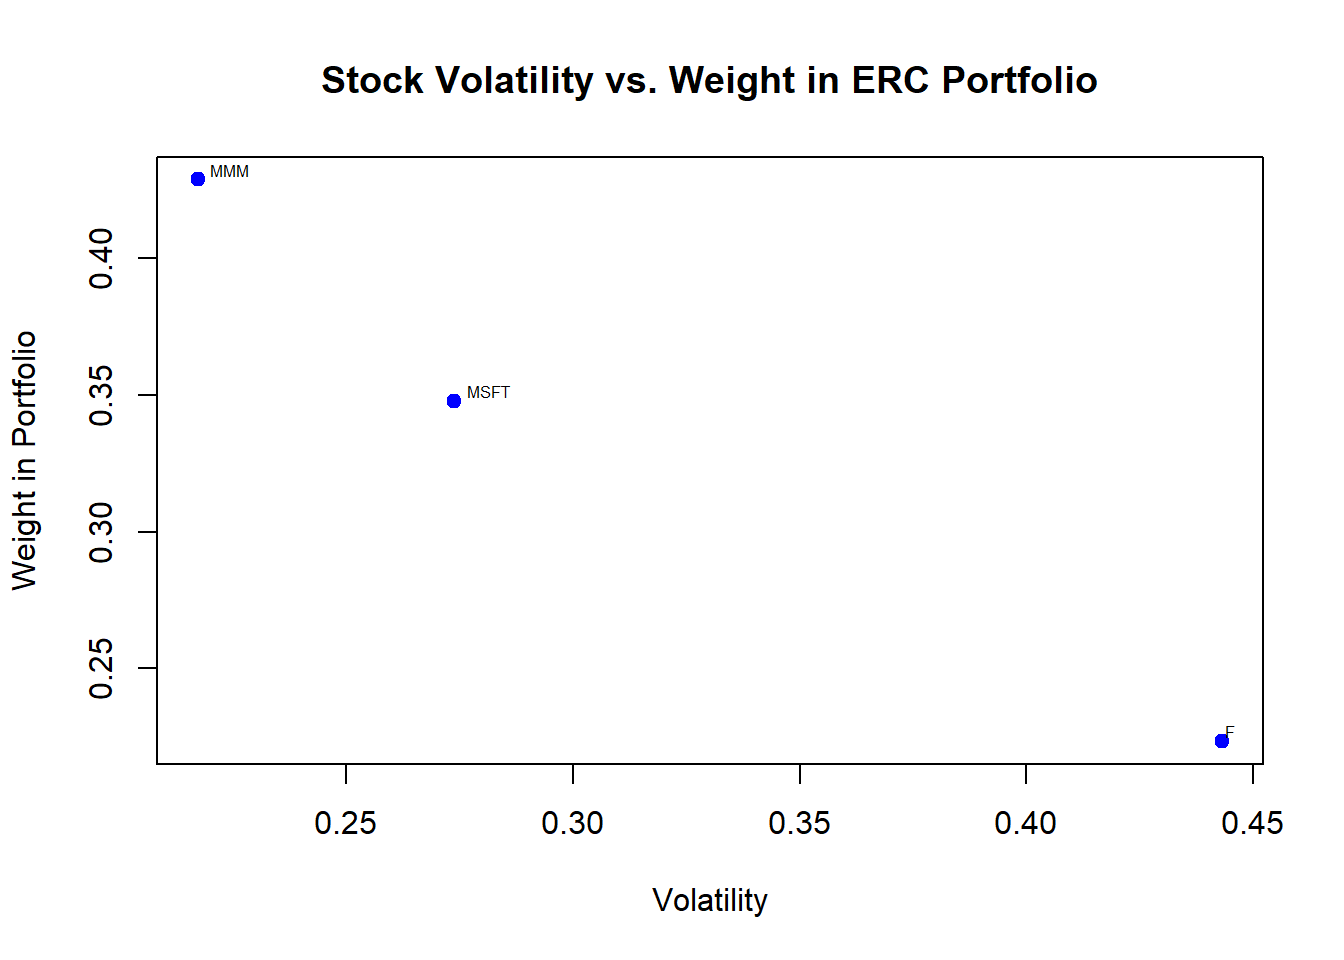
\includegraphics{mqim_book_files/figure-latex/unnamed-chunk-8-1.pdf}

\section{Concentration/Diversification}\label{concentrationdiversification}

Mean-Variance optimal portfolios are often highly concentrated, with
potentially very large positions in the most attractive assets:

\begin{Shaded}
\begin{Highlighting}[]
\KeywordTok{library}\NormalTok{(quantmod)}
\KeywordTok{library}\NormalTok{(quadprog)}
\NormalTok{tickers <-}\StringTok{ }\KeywordTok{c}\NormalTok{(}\StringTok{"MMM"}\NormalTok{,}\StringTok{"AXP"}\NormalTok{,}\StringTok{"AAPL"}\NormalTok{,}\StringTok{"BA"}\NormalTok{,}\StringTok{"CAT"}\NormalTok{,}\StringTok{"CVX"}\NormalTok{,}\StringTok{"CSCO"}\NormalTok{,}
             \StringTok{"KO"}\NormalTok{,}\StringTok{"DIS"}\NormalTok{,}\StringTok{"DWDP"}\NormalTok{,}\StringTok{"XOM"}\NormalTok{,}\StringTok{"GE"}\NormalTok{,}\StringTok{"GS"}\NormalTok{,}\StringTok{"HD"}\NormalTok{,}\StringTok{"IBM"}\NormalTok{,}
             \StringTok{"INTC"}\NormalTok{,}\StringTok{"JNJ"}\NormalTok{,}\StringTok{"JPM"}\NormalTok{,}\StringTok{"MCD"}\NormalTok{,}\StringTok{"MRK"}\NormalTok{,}\StringTok{"MSFT"}\NormalTok{,}\StringTok{"NKE"}\NormalTok{,}
             \StringTok{"PFE"}\NormalTok{,}\StringTok{"PG"}\NormalTok{,}\StringTok{"TRV"}\NormalTok{,}\StringTok{"UTX"}\NormalTok{,}\StringTok{"UNH"}\NormalTok{,}\StringTok{"VZ"}\NormalTok{,}\StringTok{"V"}\NormalTok{,}\StringTok{"WMT"}\NormalTok{)}
\KeywordTok{getSymbols}\NormalTok{(tickers)}
\end{Highlighting}
\end{Shaded}

\begin{verbatim}
##  [1] "MMM"  "AXP"  "AAPL" "BA"   "CAT"  "CVX"  "CSCO" "KO"   "DIS"  "DWDP"
## [11] "XOM"  "GE"   "GS"   "HD"   "IBM"  "INTC" "JNJ"  "JPM"  "MCD"  "MRK" 
## [21] "MSFT" "NKE"  "PFE"  "PG"   "TRV"  "UTX"  "UNH"  "VZ"   "V"    "WMT"
\end{verbatim}

\begin{Shaded}
\begin{Highlighting}[]
\NormalTok{dat <-}\StringTok{ }\NormalTok{MMM}\OperatorTok{$}\NormalTok{MMM.Adjusted}
\ControlFlowTok{for}\NormalTok{ (i }\ControlFlowTok{in} \DecValTok{2}\OperatorTok{:}\KeywordTok{length}\NormalTok{(tickers)) \{}
\NormalTok{  obj <-}\StringTok{ }\KeywordTok{paste}\NormalTok{(tickers[i],}\StringTok{"$"}\NormalTok{,tickers[i],}\StringTok{".Adjusted"}\NormalTok{,}\DataTypeTok{sep=}\StringTok{""}\NormalTok{)}
\NormalTok{  dat <-}\StringTok{ }\KeywordTok{merge}\NormalTok{(dat,}\KeywordTok{eval}\NormalTok{(}\KeywordTok{parse}\NormalTok{(}\DataTypeTok{text=}\NormalTok{obj)))}
\NormalTok{  \}}
\KeywordTok{colnames}\NormalTok{(dat) <-}\StringTok{ }\NormalTok{tickers}
\NormalTok{dat <-}\StringTok{ }\NormalTok{dat[}\StringTok{'2008-03-19/'}\NormalTok{]}

\NormalTok{ret <-}\StringTok{ }\NormalTok{(}\KeywordTok{exp}\NormalTok{(}\KeywordTok{diff}\NormalTok{(}\KeywordTok{log}\NormalTok{(dat)))}\OperatorTok{-}\DecValTok{1}\NormalTok{)[}\OperatorTok{-}\DecValTok{1}\NormalTok{,]}

\NormalTok{sigma <-}\StringTok{ }\KeywordTok{cov}\NormalTok{(ret)}

\NormalTok{exp_ret <-}\StringTok{ }\KeywordTok{array}\NormalTok{(}\DecValTok{0}\NormalTok{,}\DataTypeTok{dim=}\KeywordTok{c}\NormalTok{(}\DecValTok{30}\NormalTok{,}\DecValTok{1}\NormalTok{)) }
\NormalTok{const <-}\StringTok{ }\KeywordTok{array}\NormalTok{(}\DecValTok{1}\NormalTok{,}\DataTypeTok{dim=}\KeywordTok{c}\NormalTok{(}\DecValTok{30}\NormalTok{,}\DecValTok{1}\NormalTok{)) }
\NormalTok{Amat <-}\StringTok{ }\KeywordTok{cbind}\NormalTok{(const, }\KeywordTok{diag}\NormalTok{(}\KeywordTok{nrow}\NormalTok{(sigma)))}
\NormalTok{bvec <-}\StringTok{ }\KeywordTok{c}\NormalTok{(}\DecValTok{1}\NormalTok{, }\KeywordTok{rep}\NormalTok{(}\DecValTok{0}\NormalTok{, }\KeywordTok{nrow}\NormalTok{(sigma))) }
\NormalTok{port_wgts <-}\StringTok{ }\KeywordTok{solve.QP}\NormalTok{(sigma,exp_ret,Amat,}\DataTypeTok{bvec=}\NormalTok{bvec,}\DataTypeTok{meq=}\DecValTok{1}\NormalTok{)}\OperatorTok{$}\NormalTok{solution}
\KeywordTok{names}\NormalTok{(port_wgts) <-}\StringTok{ }\NormalTok{tickers}

\KeywordTok{barplot}\NormalTok{(port_wgts,}
        \DataTypeTok{main=}\StringTok{"Unconstrained Minimum Variance Portfolio Weights"}\NormalTok{,}
        \DataTypeTok{ylab=}\StringTok{"Weight in MVP"}\NormalTok{,}
        \DataTypeTok{las=}\DecValTok{2}\NormalTok{)}
\end{Highlighting}
\end{Shaded}

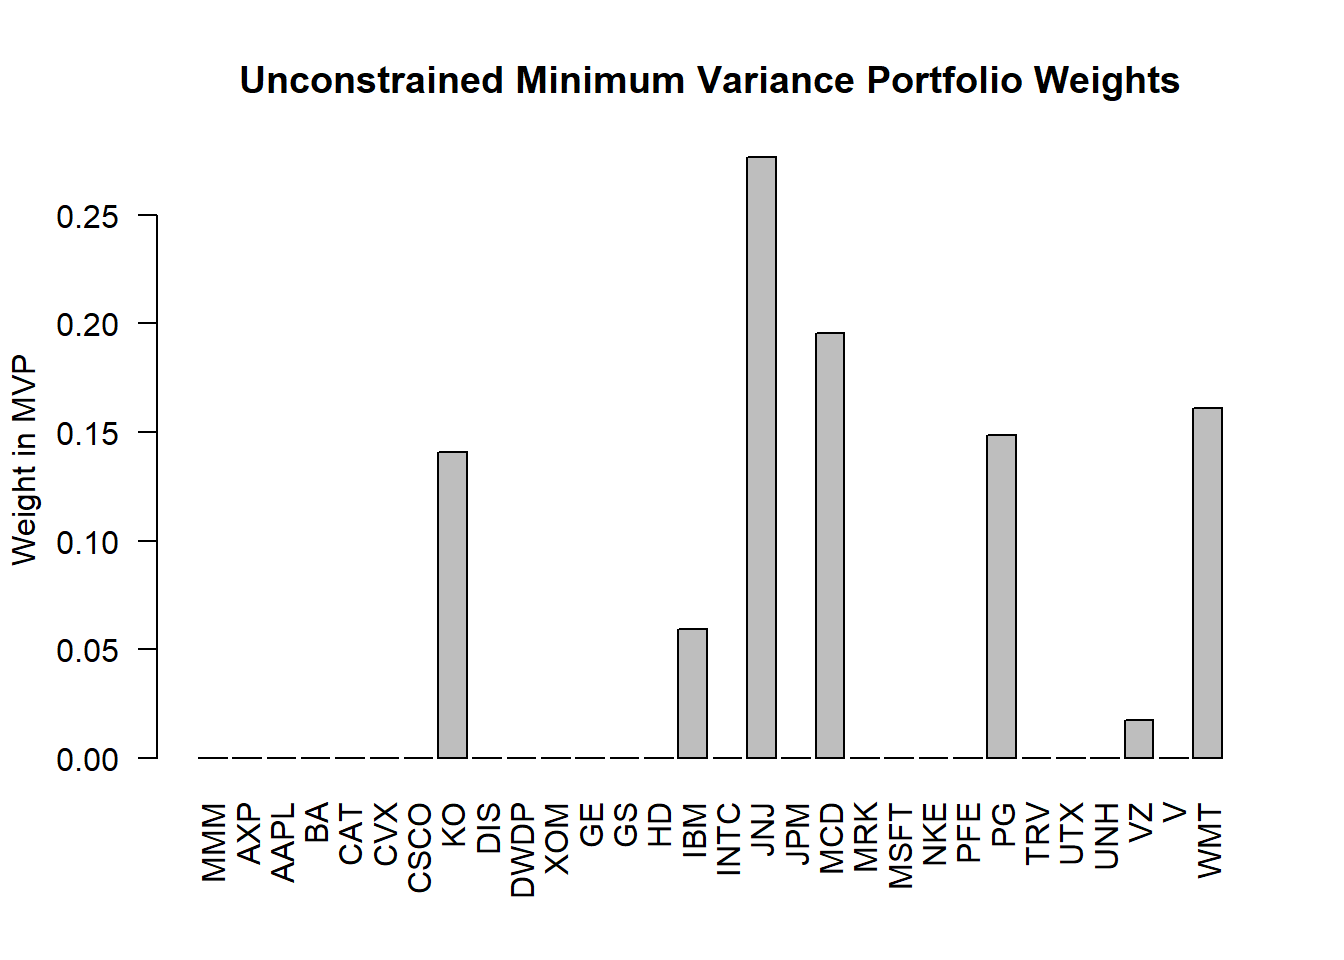
\includegraphics{mqim_book_files/figure-latex/unnamed-chunk-9-1.pdf}

Using a representative sample of 30 large cap U.S. stocks, an
unconstrained MVP results in the portfolio holding as much as 20-30\% in
certain stocks.

Two methods to prioritize diversification/deconcentration in the
optimization process include the \textbf{Most Diversified Portfolio
(``MDP'')} approach of \citep{choueifaty2008} as well as the direct
modification of the objective function using the
\textbf{Herfindahl-Hirschman Index (``HHI'')}.

\subsection{Most Diversified
Portfolio}\label{most-diversified-portfolio}

The MDP is the portfolio that maximizes the diversification ratio of the
portfolio, defined as the ratio of the weighted average volatility of
the portfolio constituents to the volatility of the portfolio:

\[
DR = \frac{\omega' v}{\sqrt{\omega' \Sigma \omega}}
\]

Where \(v\) is a vector of individual asset volatilities. Maximization
of the diversification ratio is equivalent to the following optimization
objective function:

\[
min_\omega \quad \omega' C \omega \quad \text{s.t.} \ \omega' \mathbf{1} = 1
\]

with \(C\) the correlation matrix of assets in the investment universe.

\begin{Shaded}
\begin{Highlighting}[]
\KeywordTok{library}\NormalTok{(quantmod)}
\NormalTok{tickers <-}\StringTok{ }\KeywordTok{c}\NormalTok{(}\StringTok{"F"}\NormalTok{,}\StringTok{"MMM"}\NormalTok{,}\StringTok{"MSFT"}\NormalTok{)}
\KeywordTok{getSymbols}\NormalTok{(tickers)}
\end{Highlighting}
\end{Shaded}

\begin{verbatim}
## [1] "F"    "MMM"  "MSFT"
\end{verbatim}

\begin{Shaded}
\begin{Highlighting}[]
\NormalTok{dat <-}\StringTok{ }\KeywordTok{merge.xts}\NormalTok{(F}\OperatorTok{$}\NormalTok{F.Adjusted, MMM}\OperatorTok{$}\NormalTok{MMM.Adjusted, MSFT}\OperatorTok{$}\NormalTok{MSFT.Adjusted)}
\NormalTok{ret <-}\StringTok{ }\NormalTok{(}\KeywordTok{exp}\NormalTok{(}\KeywordTok{diff}\NormalTok{(}\KeywordTok{log}\NormalTok{(dat)))}\OperatorTok{-}\DecValTok{1}\NormalTok{)[}\OperatorTok{-}\DecValTok{1}\NormalTok{,]}
\NormalTok{C <-}\StringTok{ }\KeywordTok{cor}\NormalTok{(ret)}
\NormalTok{mdp <-}\StringTok{ }\KeywordTok{as.numeric}\NormalTok{((}\KeywordTok{solve}\NormalTok{(C)}\OperatorTok\KeywordTok{rep}\NormalTok{(}\DecValTok{1}\NormalTok{,}\DecValTok{3}\NormalTok{))}\OperatorTok{/}\KeywordTok{as.numeric}\NormalTok{(}\KeywordTok{rep}\NormalTok{(}\DecValTok{1}\NormalTok{,}\DecValTok{3}\NormalTok{)}\OperatorTok\KeywordTok{solve}\NormalTok{(C)}\OperatorTok\KeywordTok{rep}\NormalTok{(}\DecValTok{1}\NormalTok{,}\DecValTok{3}\NormalTok{)))}
\KeywordTok{names}\NormalTok{(mdp) <-}\StringTok{ }\NormalTok{tickers}
\KeywordTok{barplot}\NormalTok{(mdp,}
        \DataTypeTok{main=}\StringTok{"Weights of Most Diversified Portfolio"}\NormalTok{,}
        \DataTypeTok{xlab=}\StringTok{"Stock"}\NormalTok{,}
        \DataTypeTok{ylab=}\StringTok{"Weight"}\NormalTok{)}
\end{Highlighting}
\end{Shaded}

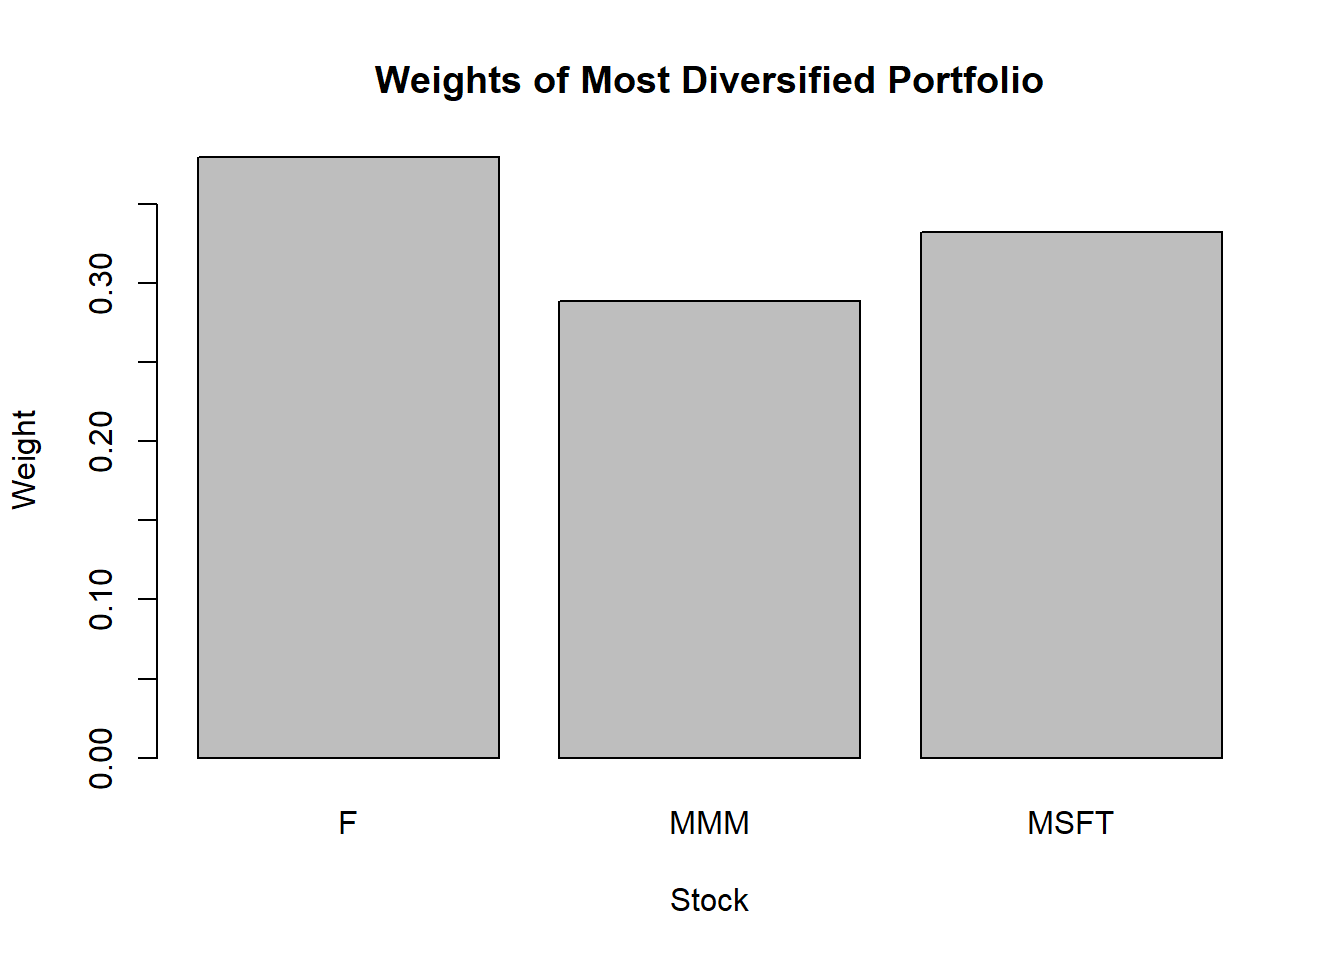
\includegraphics{mqim_book_files/figure-latex/unnamed-chunk-10-1.pdf}

\subsection{HHI Based Deconcentration}\label{hhi-based-deconcentration}

The Herfindahl-Hirschman Index (defined as
\(HHI(\omega) = \sum_{i=1}^N \omega_i^2\)) is a measure of market
concentration and was applied in a portfolio optimization context in
\citep{king2007}.The approach generalizes to that of the use of a
modified covariance matrix in the optimization objective function. For a
minimum variance portfolio with a concentration penalty:

\[
\min_\omega \quad \omega' (\Sigma + \lambda_{c} \mathbf{I}) \omega \quad \text{s.t.} \ \omega' \mathbf{1} = 1
\]

Where:

\begin{itemize}
\tightlist
\item
  \(\mathbf{I}\) is an identity matrix
\item
  \(\lambda_c\) is a \emph{concentration risk aversion} parameter
\end{itemize}

Larger values of \(\lambda_c\) produce portfolios that are less
concentrated in nature, while a value of \(\lambda_c = 0\) results in
the unconstrained minimum variance formulation (no weight given to
avoidance of concentration risk).

Using a minimum variance portfolio as an example, we can observe the
impact of a concentration penalty on the resulting weight of a 3 asset
portfolio:

\begin{Shaded}
\begin{Highlighting}[]
\KeywordTok{library}\NormalTok{(tseries)}
\KeywordTok{library}\NormalTok{(quantmod)}
\NormalTok{tickers <-}\StringTok{ }\KeywordTok{c}\NormalTok{(}\StringTok{"F"}\NormalTok{,}\StringTok{"MMM"}\NormalTok{,}\StringTok{"MSFT"}\NormalTok{)}
\KeywordTok{getSymbols}\NormalTok{(tickers)}
\end{Highlighting}
\end{Shaded}

\begin{verbatim}
## [1] "F"    "MMM"  "MSFT"
\end{verbatim}

\begin{Shaded}
\begin{Highlighting}[]
\NormalTok{dat <-}\StringTok{ }\KeywordTok{merge.xts}\NormalTok{(F}\OperatorTok{$}\NormalTok{F.Adjusted, MMM}\OperatorTok{$}\NormalTok{MMM.Adjusted, MSFT}\OperatorTok{$}\NormalTok{MSFT.Adjusted)}
\NormalTok{ret <-}\StringTok{ }\NormalTok{(}\KeywordTok{exp}\NormalTok{(}\KeywordTok{diff}\NormalTok{(}\KeywordTok{log}\NormalTok{(dat)))}\OperatorTok{-}\DecValTok{1}\NormalTok{)[}\OperatorTok{-}\DecValTok{1}\NormalTok{,]}
\NormalTok{sigma <-}\StringTok{ }\KeywordTok{cov}\NormalTok{(ret)}
\NormalTok{lambda_c <-}\StringTok{ }\KeywordTok{seq}\NormalTok{(}\DecValTok{0}\NormalTok{,}\FloatTok{0.01}\NormalTok{,}\DataTypeTok{length.out=}\DecValTok{50}\NormalTok{)}
\NormalTok{port_wgts <-}\StringTok{ }\KeywordTok{array}\NormalTok{(}\DecValTok{0}\NormalTok{,}\DataTypeTok{dim=}\KeywordTok{c}\NormalTok{(}\DecValTok{3}\NormalTok{,}\DecValTok{50}\NormalTok{))}
\ControlFlowTok{for}\NormalTok{ (i }\ControlFlowTok{in} \DecValTok{1}\OperatorTok{:}\KeywordTok{dim}\NormalTok{(port_wgts)[}\DecValTok{2}\NormalTok{]) \{}
\NormalTok{  sigma_adj <-}\StringTok{ }\NormalTok{sigma }\OperatorTok{+}\StringTok{ }\NormalTok{lambda_c[i]}\OperatorTok{*}\KeywordTok{diag}\NormalTok{(}\DecValTok{3}\NormalTok{)}
\NormalTok{  port_wgts[,i] <-}\StringTok{ }\NormalTok{\{(}\KeywordTok{solve}\NormalTok{(sigma_adj)}\OperatorTok\KeywordTok{rep}\NormalTok{(}\DecValTok{1}\NormalTok{,}\DecValTok{3}\NormalTok{))}\OperatorTok{/}
\StringTok{      }\KeywordTok{as.numeric}\NormalTok{(}\KeywordTok{rep}\NormalTok{(}\DecValTok{1}\NormalTok{,}\DecValTok{3}\NormalTok{)}\OperatorTok\KeywordTok{solve}\NormalTok{(sigma_adj)}\OperatorTok\KeywordTok{rep}\NormalTok{(}\DecValTok{1}\NormalTok{,}\DecValTok{3}\NormalTok{))\}}
\NormalTok{\}}
\KeywordTok{colnames}\NormalTok{(port_wgts) <-}\StringTok{ }\KeywordTok{as.character}\NormalTok{(}\KeywordTok{round}\NormalTok{(lambda_c,}\DataTypeTok{digits=}\DecValTok{3}\NormalTok{))}
\KeywordTok{par}\NormalTok{(}\DataTypeTok{mar=}\KeywordTok{c}\NormalTok{(}\FloatTok{5.1}\NormalTok{, }\FloatTok{4.1}\NormalTok{, }\FloatTok{4.1}\NormalTok{, }\FloatTok{8.1}\NormalTok{), }\DataTypeTok{xpd=}\OtherTok{TRUE}\NormalTok{)}
\KeywordTok{barplot}\NormalTok{(port_wgts,}
        \DataTypeTok{main=}\StringTok{"Effect of Concentration Penalty on }\CharTok{\textbackslash{}n}\StringTok{ Minimum Variance Portfolio Weights"}\NormalTok{,}
        \DataTypeTok{xlab=}\StringTok{"Value of Concentration Risk Aversion Parameter"}\NormalTok{,}
        \DataTypeTok{ylab=}\StringTok{"Weight"}\NormalTok{,}
        \DataTypeTok{col=}\KeywordTok{c}\NormalTok{(}\StringTok{"grey"}\NormalTok{,}\StringTok{"lightblue"}\NormalTok{,}\StringTok{"lightgreen"}\NormalTok{)}
\NormalTok{        )}
\KeywordTok{legend}\NormalTok{(}\StringTok{"topright"}\NormalTok{, }\DataTypeTok{inset=}\KeywordTok{c}\NormalTok{(}\OperatorTok{-}\FloatTok{0.2}\NormalTok{,}\DecValTok{0}\NormalTok{), }\DataTypeTok{legend=}\NormalTok{tickers,}\DataTypeTok{col=}\KeywordTok{c}\NormalTok{(}\StringTok{"grey"}\NormalTok{,}\StringTok{"lightblue"}\NormalTok{,}\StringTok{"lightgreen"}\NormalTok{),}\DataTypeTok{lty=}\DecValTok{1}\NormalTok{)}
\end{Highlighting}
\end{Shaded}

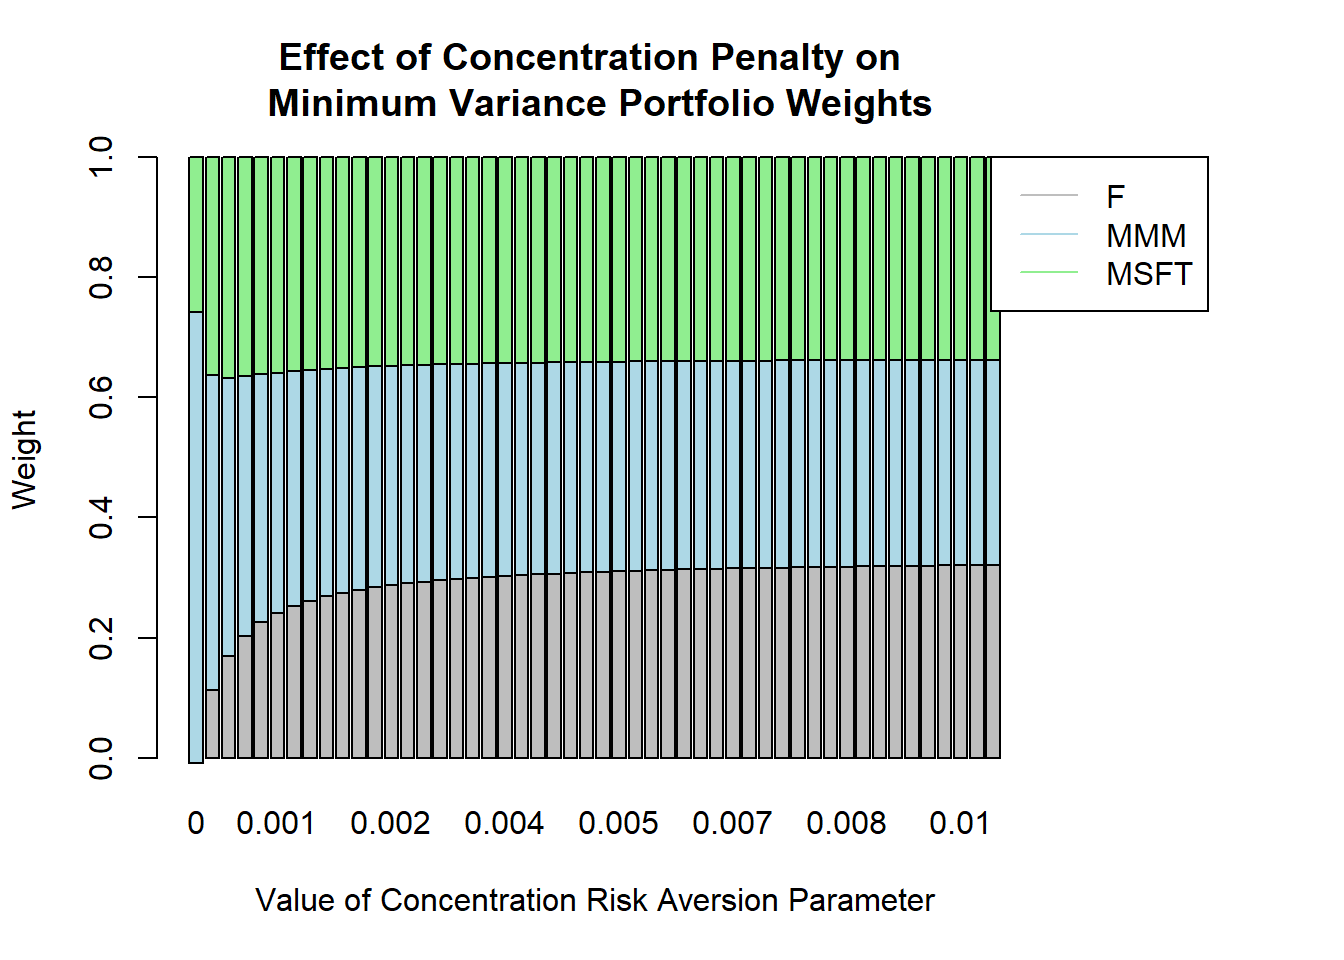
\includegraphics{mqim_book_files/figure-latex/unnamed-chunk-11-1.pdf}

\section{Mean-CVaR}\label{mean-cvar}

While the standard MPT optimization approach uses variance as the
measure of risk in the objective function:

\[
\max_\omega \quad \omega' \mu - \frac{1}{2} \lambda \omega' \Sigma \omega
\]

\citep{rockafellar2000} replaced variance with the downside risk measure
\textbf{Conditional Value-at-Risk (``CVaR'')} - sometimes referred to as
Expected Tail Loss (``ETL''):

\[
CVaR_\alpha = - \mathbb{E} (r|r \leq q^r(\alpha))
\]

Aplying this in a quadratic utility framework results in the objective
function

\[
\max_\omega \quad \omega' \mu -  \lambda \cdot \text{CVaR}_\alpha (\omega) \quad \text{s.t.} \ \omega' \mathbf{1} = 1
\]

(TODO): Finish CVaR Section with example

\section{Synthesis of PMPT
Approaches}\label{synthesis-of-pmpt-approaches}

(TODO): Results from paper showing optimality, etc., reasons why for
each approach.

\chapter*{Appendix 1 - Special Topics}\label{appendix1}
\addcontentsline{toc}{chapter}{Appendix 1 - Special Topics}

TBC

\section*{Hedge Fund Replication}\label{hedge-fund-replication}
\addcontentsline{toc}{section}{Hedge Fund Replication}

TBC

\section*{Robustness}\label{robustness}
\addcontentsline{toc}{section}{Robustness}

TBC

\chapter*{Appendix 2 - Background Information}\label{appendix2}
\addcontentsline{toc}{chapter}{Appendix 2 - Background Information}

\section*{Matrix Algebra Review}\label{matrix-algebra-review}
\addcontentsline{toc}{section}{Matrix Algebra Review}

Basic portfolio mathematics is much easier to understand (and write
clearly) if the reader has understanding of some simple matrix algebra
techniques. For example, the variance \(\sigma_p^2\) of portfolio of two
assets written out in fully expanded form is often expressed as the sum
of three separate terms:

\begin{equation}
\sigma_p^2 = \omega_1^2 \sigma_1^2 + \omega_2^2 \sigma_2^2 + 2 \omega_1 \omega_2 \sigma_2 \sigma_2 \rho_{1,2}
\end{equation}

For a three asset portfolio, we need to take the sum of six separate
terms (in fact, for \(n\) assets, we would have to take the sum of
\(\frac{n(n+1)}{2}\) terms). Conversely, in matrix language this would
be written as simply \(\sigma_p^2 = \omega' \Sigma \omega\) irrespective
of the number of assets in the portfolio.

This appendix covers the very basics of matrix mathematics required to
understand the above and succeeed in this class - including basic matrix
computational techniques and an introduction to finding inverse
matrices. Further coverage is available in Dr.~Eric Zivot's \emph{Matrix
Algebra Review} available at
\url{http://faculty.washington.edu/ezivot/econ424/matrixreview.pdf}, or
alternatively for a textbook treatment, the first few chapters of Chiang
et al \emph{Fundamental Methods of Mathematical Economics} contains most
of what would be necessary for this course.

\subsection*{Basic Concepts}\label{basic-concepts}
\addcontentsline{toc}{subsection}{Basic Concepts}

Matrix addition is defined for same-dimension matrices:

\[
\begin{bmatrix} 1 & 4 \\ 3 & 7 \end{bmatrix} + 
\begin{bmatrix} 2 & 3 \\ 1 & 1 \end{bmatrix} = 
\begin{bmatrix} 3 & 7 \\ 4 & 8 \end{bmatrix}
\]

A matrix can be multiplied by a scalar by multiplying that scalar by
each element of the matrix:

\[
2 \times 
\begin{bmatrix} 2 & 3 \\ 1 & 1 \end{bmatrix} = 
\begin{bmatrix} 4 & 6 \\ 2 & 2 \end{bmatrix}
\]

The dot-product of two conformable vectors is the sum of the
corresponding elements multiplied together:

\[
\begin{bmatrix} 1 & 4  \end{bmatrix} \times 
\begin{bmatrix} 2 \\ 1 \end{bmatrix} = 
1 \times 2 + 4 \times 1 =
6
\]

Matrix multiplication is defined in a similar way, in that matrices are
conformable when the number of columns in the first matrix is the same
as the number of rows in the second:\textbackslash{}

\[
\begin{bmatrix} 1 & 4 \\ 3 & 7 \end{bmatrix} \times 
\begin{bmatrix} 2 & 3 \\ 1 & 1 \end{bmatrix} = 
\begin{bmatrix} 1 \times 2 + 4 \times 1 & 1 \times 3 + 4 \times 1 \\ 3 \times 2 + 7 \times 1 & 3 \times 3 + 7 \times 1 \end{bmatrix} = 
\begin{bmatrix} 6 & 7 \\ 13 & 16 \end{bmatrix}
\]

Division of matrices is not concept that is defined, although a similar
idea is contained within the concept of inverse matrices.

\subsection*{Inverse Matrices}\label{inverse-matrices}
\addcontentsline{toc}{subsection}{Inverse Matrices}

The Identity Matrix \(I\) is simply a matrix with 1's in the diagonal
elements and 0's elsewhere:

\[
\begin{bmatrix} 1 & 0 & 0 \\ 0 & 1 & 0 \\ 0 & 0 & 1 \end{bmatrix}
\]

If you check, you can see that any matrix \(X\) multiplied with the
Identity matrix results in the original matrix \(X\) - that is,
\(XI = IX = X\) and \(II = I\). Another interesting matrix is that of
the Inverse matrix. For any matrix \(X\), its inverse is denoted
\(X^{-1}\), and an any matrix multiplied by its inverse results in the
Identity Matrix - that is, \(XX^{-1} = X^{-1}X = I\). This is therefore
analogous to division for matrices, and will prove to be useful.

Now, consider a system of equations - three equations and three unknowns
- below:

\begin{align*} 
3x_1 + 5x_2 + x_3 &= 29 \\ 
7x_1 + 2x_2 + 4x_3 &= 60 \\ 
-6x_1 + 3x_2 + 2x_3 &= -4 
\end{align*}

How can we solve this system of equations (that is, find the values of
\(x_1, x_2, x_3\) that make the left and right hand sides equal)? The
method of Gauss-Jordan elimination is often taught, but this is tedious
even for \(3 \times 3\) systems (there are shortcut methods for
\(2 \times 2\) matrices), and so we ignore the details behind it and
skip forward to computational implementations. It turns out that we can
re-write the system equations as follows in matrix form, and that
through the use of the inverse matrix, we can easily solve such a
system. If we write:

\[
A = \begin{bmatrix} 3 & 5 & 1 \\ 7 & 2 & 4 \\ -6 & 3 & 2\end{bmatrix}  
x = \begin{bmatrix} x_1  \\ x_2 \\ x_3 \end{bmatrix} 
b = \begin{bmatrix} 29 \\ 60 \\ 4 \end{bmatrix}
\]

Then the equivalent system in matrix form is written \(Ax = b\). The
question is how to find the values of \(x\) that make \(Ax = b\).
Because of the properties of the Identity Matrix \(I\) and the Inverse
Matrix we defined above, we are able to take the following steps:

\begin{align*}
Ax &= b \\
A^{-1}Ax &= A^{-1}b \\
Ix &= A^{-1}b\\
x &= A^{-1}b
\end{align*}

And so we can solve any such system of equations (provided a solution
exists, which is essentially equivalent to the existence of the Inverse
Matrix for the Matrix \(A\)) by simply pre-multiplying the \(b\) vector
by the matrix \(A^{-1}\).

Note that in R, it is often recommended to use the \textit{solve()}
function to find the matrix inverse. You can verify the above in R as
follows:

\begin{Shaded}
\begin{Highlighting}[]
\NormalTok{(}\DataTypeTok{A =} \KeywordTok{matrix}\NormalTok{(}\KeywordTok{c}\NormalTok{(}\DecValTok{3}\NormalTok{, }\DecValTok{5}\NormalTok{, }\DecValTok{1}\NormalTok{, }\DecValTok{7}\NormalTok{, }\DecValTok{2}\NormalTok{, }\DecValTok{4}\NormalTok{, }\OperatorTok{-}\DecValTok{6}\NormalTok{, }\DecValTok{3}\NormalTok{, }\DecValTok{2}\NormalTok{),}\DataTypeTok{nrow=}\DecValTok{3}\NormalTok{,}\DataTypeTok{byrow=}\NormalTok{T))}
\end{Highlighting}
\end{Shaded}

\begin{verbatim}
##      [,1] [,2] [,3]
## [1,]    3    5    1
## [2,]    7    2    4
## [3,]   -6    3    2
\end{verbatim}

\begin{Shaded}
\begin{Highlighting}[]
\NormalTok{(}\DataTypeTok{b =} \KeywordTok{matrix}\NormalTok{(}\KeywordTok{c}\NormalTok{(}\DecValTok{29}\NormalTok{,}\DecValTok{60}\NormalTok{,}\OperatorTok{-}\DecValTok{4}\NormalTok{),}\DataTypeTok{nrow=}\DecValTok{3}\NormalTok{,}\DataTypeTok{byrow=}\NormalTok{T))}
\end{Highlighting}
\end{Shaded}

\begin{verbatim}
##      [,1]
## [1,]   29
## [2,]   60
## [3,]   -4
\end{verbatim}

\begin{Shaded}
\begin{Highlighting}[]
\NormalTok{(A.inv <-}\StringTok{ }\KeywordTok{solve}\NormalTok{(A))}
\end{Highlighting}
\end{Shaded}

\begin{verbatim}
##            [,1]        [,2]        [,3]
## [1,]  0.0441989  0.03867403 -0.09944751
## [2,]  0.2099448 -0.06629834  0.02762431
## [3,] -0.1823204  0.21546961  0.16022099
\end{verbatim}

\begin{Shaded}
\begin{Highlighting}[]
\NormalTok{(x <-}\StringTok{ }\NormalTok{A.inv }\OperatorTok\StringTok{ }\NormalTok{b)}
\end{Highlighting}
\end{Shaded}

\begin{verbatim}
##      [,1]
## [1,]    4
## [2,]    2
## [3,]    7
\end{verbatim}

And in fact we get the proper solution of \(x = (4, 2, 7)\), that is,
\(x_1 = 4, x_2 = 2, x_3 = 7\).

\subsection*{Sums}\label{sums}
\addcontentsline{toc}{subsection}{Sums}

However, despite the fact that we will use matrices whenever
appropriate, there are times when it is useful or more intuitive to use
sums instead. For example, the sum of all integers from 1 to 100 could
be written in summation notation as:

\begin{align*}
1 + 2 + ... + 100 = \displaystyle\sum_{i=1}^{100} i
\end{align*}

Often, expressions can be written equivalently suing summation notation
or using matrix notation, and we will often find summation notation
convenient, particularly when encountering concepts like risk
decomposition for the first time. For the purposes of this text, it will
be helpful to remember that:

\begin{itemize}
\tightlist
\item
  \(\textbf{c}'\textbf{x} = \displaystyle\sum_{i=1}^{n} c_i x_i\) when
  \textbf{c} and \textbf{x} are vectors of length \(n\)
\item
  \(\textbf{c}' \textbf{X} \textbf{c} = \displaystyle\sum_{i=1}^{n} \displaystyle\sum_{j=1}^{n} c_i c_j X_{i,j}\)
  when \textbf{c} is a vector of length \(n\) and \(X\) is an
  \(n \times n\) matrix
\end{itemize}

\section*{Probability Review}\label{probability-review}
\addcontentsline{toc}{section}{Probability Review}

This section covers only the bare minimum of the very basics of
probability and expectation that is needed to complete this course. For
a good probability review that does assume some prior knowledge, consult
Eric Zivot's \emph{Probability Review} available at
\url{http://faculty.washington.edu/ezivot/econ424/probreview.pdf}. For
more in depth coverage beginning with the basics in a textbook-like
format, Grinstead and Snell's \emph{Introduction to Probability}
\citep{gs2006} is a good choice and is available free online.

\subsection*{Probability Distributions \& Random
Variables}\label{probability-distributions-random-variables}
\addcontentsline{toc}{subsection}{Probability Distributions \& Random
Variables}

A Random Variable \(X\) (hereafter: R.V.) is a function that maps each
outcome from a sample space into a real number. For example, in the case
of tossing a regular 6-sided die, the R.V. could take the values (1, 2,
3, 4, 5, 6).

A Probability Mass Function (hereafter: PMF) is a function \(f_X(x)\)
that maps the values of a R.V. \(X\) on to numbers between 0 and 1,
inclusive. That is, the PMF gives the probability of the outcome of the
R.V. occurring:

\begin{equation}
f_X(x) = \mathbb{P}(X = x)
\end{equation}

Which can be read as ``the probability that the R.V. X takes on the
value \(x\)'' (there are similar definitions for continuous R.V.'s,
although we ignore them for this class). Using this definition, we can
also define the cumulative probability mass as:

\begin{equation}
F_X(x) = \sum\limits_{i=1}^n \mathbb{P}(X = x_i)
\end{equation}

Where the total sum of all possible non-overlapping events in the sample
space amounts to \(\mathbb{P}(\Omega) = 1\).

\subsection*{Rules of Expectation \&
Variance}\label{rules-of-expectation-variance}
\addcontentsline{toc}{subsection}{Rules of Expectation \& Variance}

For a discrete random variable, we interpret the Expected Value
(\(\mathbb{E}\)) of that random variable to be its average value in
repeated sampling, and it is defined as the probability weighted sum of
all possible outcomes. In mathematical notation, the expectation of the
R.V. \(X\) is:

\begin{equation}
\mathbb{E}X = \sum\limits_{i=1}^n x_i * \mathbb{P}(X=x_i)
\end{equation}

For \(n\) equally likely events, this can be simplified to:

\begin{equation}
\mathbb{E}X = \frac{1}{n} * (\sum\limits_{i=1}^n x_i)
\end{equation}

For example, if we define a random variable \(X\) that pays \$1 if a
(fair) coin comes up as heads, and -\$1 if the coin comes up as tails,
then the expected value of that random variable is:

\begin{align*}
\mathbb{E}(X) &= \frac{1}{2}*1 + \frac{1}{2}*(-1)\\
&= \frac{1}{2} * (1 + (-1))\\
&= 0\\
\end{align*}

There are various rules of expectations that we should know:

\begin{itemize}
\tightlist
\item
  The expected value of a constant \(c\) is that constant:
  \(\mathbb{E}(c) = c\)
\item
  The expected value of a random variable \(X\) plus a constant \(c\) is
  the expected value of the random variable plus the constant:
  \(\mathbb{E}(X + c) = \mathbb{E}(X) + c\)
\item
  The expected value of a constant \(a\) multiplied by a random variable
  \(X\) is the constant multiplied by the expectation of the random
  variable: \(\mathbb{E}(aX) = a\mathbb{E}(X)\)\textbackslash{}
\end{itemize}

In addition, there are other rules of expectation that are important to
know, but not necessarily for this course, and so they are omitted.
However, we also need to be aware of some similar rules or properties
for variance and co-variance. Recall that the definition of the variance
of a random variable is:

\begin{equation}
Var(X) = \mathbb{E}[(X - \mu_X)^2]
\end{equation}

Properties:

\begin{itemize}
\tightlist
\item
  \(Var(X + c) = Var(X)\)
\item
  \(Var(aX) = a^2 Var(X)\)\textbackslash{}
\end{itemize}

And likewise, the co-variance of two discrete random variables \(X\) and
\(Y\) is:

\begin{equation}
Cov(X,Y) = \mathbb{E}[(X-\mu_X)(Y-\mu_Y)]
\end{equation}

For which the following properties exist:

\begin{itemize}
\tightlist
\item
  \(Cov(X+a,Y+b) = Cov(X,Y)\)
\item
  \(Cov(aX,bY) = abCov(X,Y)\)\textbackslash{}
\end{itemize}

And this in turn allows us to define the following rules:

\begin{itemize}
\tightlist
\item
  \(Var(X + Y) = Var(X) + Var(Y) + 2*Cov(X,Y)\)
\item
  \(Var(\omega_1 X + (1-\omega_1)Y) = \omega_1^2 Var(X) + (1 - \omega_1)^2 Var(Y) + 2* \omega_1 (1 - \omega_1) Cov(X,Y)\)
\end{itemize}

Rule 2 should look familiar to anyone who has seen the expression for
the variance of a 2 asset portfolio.

The variance of a random variable \(X\) is often denoted as
\(\sigma_X^2\) in many applications, and we should remember that the
standard deviation is just the square root of the variance
\(\sigma_X = \sqrt{Var(X)}\). Finally, note that the correlation
coefficient \(\rho\) is defined as:

\begin{equation}
\rho_{X,Y} = \frac{Cov(X,Y)}{\sqrt{Var(X)Var(Y)}}
\end{equation}

\section*{Calculus Review}\label{calculus-review}
\addcontentsline{toc}{section}{Calculus Review}

In this course, we use calculus primarily to motivate the concept of
portfolio optimization. Consequently we are concerned primarily with the
concept of the derivative (of multivariate functions) and of the
techniques of optimization. These topics are briefly reviewed here here
in a highly informal/non-rigorous way. For a more complete but easy to
follow treatment of some applications that are necessary for this class,
please consult a textbook such as Chiang and Wainwright's
\emph{Fundamental Methods of Mathematical Economics}.

\subsection*{Differentiation of Vector \& Matrix Valued
Functions}\label{differentiation-of-vector-matrix-valued-functions}
\addcontentsline{toc}{subsection}{Differentiation of Vector \& Matrix
Valued Functions}

For functions of one variable, there are standard computational
techniques for obtaining derivatives. For example, for powers of \(x\):

\begin{align*}
f(x) &= 3x^3 + 2x - 8\\
f'(x) &= 9x^2 + 2\\
f''(x) &= 18x\\
f^{(3)}(x) &= 18
\end{align*}

More a slightly more complicated function such as \(y = 4(x^2-2)^3\), we
can use the \textit{chain rule}. If we let \(u = x^2 - 2\):

\begin{align*}
y(u) &= 4u^3\\
\frac{dy}{dx} &= \frac{dy}{du}\frac{du}{dx}\\
&= (12u^2)(2x)\\
&= 24x(x^2 - 2)^2
\end{align*}

In the case when we have a function of more than one variable, we take
\emph{partial} derivatives by treating all variables that are not of
interest as constants. Given a function like
\(f(x_1,x_2,x_3) = 2x^2_1 x_2x_3 + 4x_1 x_2^2 + 3x_2 + 4x^2_3\), we
would denote the first derivative w.r.t. \(x_1\) as
\(f_{x_1}(x_1,x_2,x_3)\), the first derivative w.r.t \(x_2\) as
\(f_{x_2}(x_1,x_2,x_3)\), and the first derivative w.r.t \(x_3\) as
\(f_{x_3}(x_1,x_2,x_3)\). Two successive differentiations with respect
to \(x_1\) would be labeled \(f_{x_1x_1}(x_1,x_2,x_3)\). Alternatively,
we are likely to use alternative notation such as
\(\frac{\partial y}{\partial x_1}\) or
\(\frac{\partial^2 y}{\partial x_1^2}\) to represent the first and
second derivatives w.r.t. to \(x_1\), and
\(\frac{\partial^2 y}{\partial x_1 \partial x_2}\) to be the partial
second derivative with respect to \(x_1\) and then \(x_2\). For example:

\begin{align*}
f(x_1,x_2,x_3) &= 2x^2_1 x_2x_3 + 4x_1 x_2^2 + 3x_2 + 4x^2_3\\
f_{x_1} &= 4x_1 x_2 x_3 + 4 x^2_2\\
f_{x_2} &= 2x^2_1x_3 + 8x_1 x_2 + 3\\
f_{x_3} &= 2x_1^2x_2 + 8x_3\\
f_{x_1 x_2} &= 4x_1 x_3 + 8x_2\\
\end{align*}

And so on.

Given the following:

\[
a = \begin{bmatrix} a_1 \\ a_2 \\ ... \\ a_n \end{bmatrix}, \quad x = \begin{bmatrix} x_1 \\ x_2 \\ ... \\ x_n \end{bmatrix}
\]

Then:

\begin{equation}
\label{vec_calc}
\frac{\partial}{\partial x}a'x = 
\begin{bmatrix} \frac{\partial}{\partial x_1} a_1x_1 & \frac{\partial}{\partial x_2} a_2x_2 & ... & \frac{\partial}{\partial x_n} a_nx_n \end{bmatrix} 
= a' 
\end{equation}

Given additionally:

\[
A = \begin{bmatrix} a_{1,1} & \sigma_{1,2} = a_{2,1} & ... & a_{1,n} = a_{n,1} \\
                         a_{2,1} = a_{1,2} & a_{2,2} & ... & a_{2,n} = a_{n,2} \\
                         ... & ... & ... & ... \\
                         a_{n,1} = a_{1,n} & a_{n,2} = a_{2,n} & ... & a_{n,n} \\
                         \end{bmatrix}
\]

Then:

\begin{equation}
\label{vec_calc2}
\frac{\partial}{\partial x} Ax = A 
\end{equation}

\begin{equation}
\label{vec_calc3}
\frac{\partial}{\partial x} x' A x = 2Ax
\end{equation}

This final rule will prove very useful in aspects of simple portfolio
optimization.

\subsection*{Maximization \&
Minimization}\label{maximization-minimization}
\addcontentsline{toc}{subsection}{Maximization \& Minimization}

Given a function, such as \(f(x) = -2x^2 + 5\), we find the critical
points of \(f\) by differentiating w.r.t. the decision variable (in this
case, \(x\)) and setting the first derivative equal to zero and solving
for the location:

\begin{align*}
f(x) &= -2(x-2)^2 + 5\\
f'(x) &= -4(x-2)\\
0 &= -4(x-2)\\
x &= 2
\end{align*}

And so the critical point of the original function \(f\) occurs when
\(x=2\), which would be at the point \((2,5)\).

We decide whether the critical point \((2,5)\) is a minimum or maximum
by investigating the sign of the second derivative - a negative second
derivative indicates that this is a maximum, while a positive second
derivative indicates that this is a minimum. In the case of the function
\(f\), the critical point is a maximum, since \(f''(x) = -4\).

There are similar rules for multivariable functions as well.

\subsection*{Constrained Maximization \&
Minimization}\label{constrained-maximization-minimization}
\addcontentsline{toc}{subsection}{Constrained Maximization \&
Minimization}

In most applications of maximization and minimization, we would like to
be able to constrain the decision variable in some way. Consider the
following:

\[
max_\omega \quad \omega' \Sigma \omega
\] Which is the objective function for a global minimum variance
portfolio. The unconstrained solution for this problem is found when:

\begin{align*}
\frac{\partial}{\partial \omega} \omega' \Sigma \omega &= 2 \Sigma \omega \\
F.O.C. \quad 0 &= 2 \Sigma \omega \\
0 &= \omega
\end{align*}

Or, in english, the portfolio variance is minimized when all weights are
0. This is uninteresting, and usually we with to find the minimum
variance portfolio weights in the case of \emph{full investment} wherein
the portfolio weights sum to 1, which we can represent in matrix
language with \(\omega' \mathbf{1} = 1\). We can add this constraint via
the lagrangian \(1 - \omega' \mathbf{1} = 0\). We now have the objective
function:

\[
max_\omega \quad \omega' \Sigma \omega \quad \text{s.t.} \ \omega' \mathbf{1} = 1
\]

With f.o.c.:

\[
\frac{\partial}{\partial \omega} \ [\frac{1}{2} \omega' \Sigma \omega + (1 - \omega' \mathbf{1})] = 0
\]

Solution to this will yield the (more interesting) minimum variance
portfolio with full investment:

\[
\omega^* = \frac{\Sigma^{-1} \mathbf{1}}{\mathbf{1}' \Sigma^{-1} \mathbf{1}}
\]

\bibliography{book.bib,packages.bib}


\end{document}
